\documentclass{article}

\usepackage[latin1]{inputenc}
\usepackage{tikz}

\begin{document}
\pagestyle{empty}

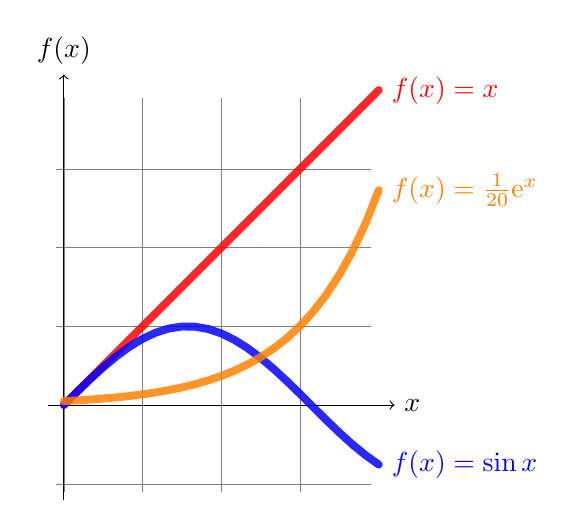
\begin{tikzpicture}
    \begin{scope}[domain=0:4]
        \draw[very thin,color=gray] (-0.1,-1.1) grid (3.9,3.9);
        \draw[->] (-0.2,0) -- (4.2,0) node[right] {$x$};
        \draw[->] (0,-1.2) -- (0,4.2) node[above] {$f(x)$};
        \draw[color=red, line width=1mm, line cap=round, opacity=0.84] plot (\x,\x) node[right, opacity=1] {$f(x) =x$};
        \draw[color=blue, line width=1mm, line cap=round, opacity=0.84] plot (\x,{sin(\x r)}) node[right, opacity=1] {$f(x) = \sin x$};
        \draw[color=orange, line width=1mm, line cap=round, opacity=0.84] plot (\x,{0.05*exp(\x)}) node[right, opacity=1] {$f(x) = \frac{1}{20} \mathrm e^x$};
    \end{scope}
\end{tikzpicture}

\end{document}
